\chapter{Systèmes d'équations linéaires}

%
%%%%%%%%%%%%%%%%%%%%%%%%%%%%%%%%%%%%%%%%%%%%%%%%%%%%
\section{Introduction}

Dans ce chapitre, nous allons voir une méthode systématique de résolution
des équations linéaires, appelée méthode d'\textbf{élimination de Gauss-Jordan}%
\footnote{Bien que l'on nomme cette méthode d'après Gauss, né en 1777, et Jordan, né en 1842, 
les mathématiciens Chinois connaissaient cette méthode au premier siècle de notre ère \ldots
et même possiblement au deuxième siècle {\bfseries avant} notre ère, 
soit plus de 2000 ans avant la naissance de Gauss.}\index{élimination de Gauss-Jordan}.
Cette méthode peut être adaptée aux matrices et, comme on le verra dans le chapitre
suivant, être utilisée pour trouver l'inverse d'une matrice.  
De plus, cette méthode peut être adaptée sous forme d'algorithme informatique
permettant d'écrire des logiciels qui peuvent résoudre des systèmes d'équations linéaires.
%
\begin{marginfigure}
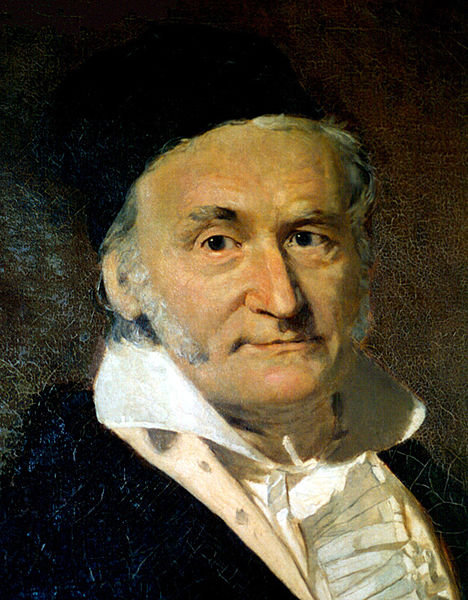
\includegraphics[width=1.8in]{images/gauss.jpg}
\caption{Johann Carl Friedrich Gauss, 1777--1855.  Surnommé le prince des mathématiques,
Gauss a laissé sa marque dans plusieurs branches des mathématiques dont,
entre autres, l'algèbre linéaire.}\label{image:gauss}
\end{marginfigure}
%

\section{Élimination de Gauss-Jordan}
Comme on l'a vu au chapitre précédent, un système de $m$ équations linéaires
et $n$ inconnues
\begin{equation}
	\begin{matrix}
	a_{11}x_1 &+& a_{12}x_2 &+& \ldots &+& a_{1n}x_n &=& b_1 \\
	a_{21}x_1 &+& a_{22}x_2 &+& \ldots &+& a_{2n}x_n &=& b_2 \\
	\vdots && \vdots &&  && \vdots && \vdots \\
	a_{m1}x_1 &+& a_{m2}x_2 &+& \ldots &+& a_{mn}x_n &=& b_m
	\end{matrix}\label{systeme}
\end{equation}
peut être écrit comme une équation matricielle $\matA\matX = \matB$
c'est-à-dire:
\[
\begin{pmatrix}
a_{11} & a_{12} & \ldots & a_{1n}\\
a_{21} & a_{22} & \ldots & a_{2n} \\
\vdots & \vdots & \vdots & \vdots \\
a_{m1} & a_{m2} & \ldots & a_{mn}
\end{pmatrix}
\begin{pmatrix}
x_1 \\ x_2 \\ \vdots \\ x_n
\end{pmatrix}
=
\begin{pmatrix}
b_1 \\ b_2 \\ \vdots \\ b_n
\end{pmatrix}
\]

On appelle la matrice $\matA$ la \definition{matrice des coefficients} du système d'équations
linéaires.

Comme on l'a vu dans le chapitre précédent, on obtiendra un système équivalent si on
effectue des \definition{opérations élémentaires sur les lignes}, soit:
\begin{itemize}
	\item[$\bullet$] on échange deux lignes :  $ L_i \leftrightarrow L_j$
	\item[$\bullet$] on remplace une ligne donnée par son multiple
	$ \alpha L_i  \quad \mbox{avec} \quad\alpha \ne 0$
	\item[$\bullet$] on remplace une ligne donnée par l'addition de celle-ci avec le multiple d'une autre ligne
	$L_i + \beta L_j \rightarrow L_i$
\end{itemize}
Dans l'exemple suivant, nous allons utiliser ces opérations élémentaires sur les lignes d'abord pour
mettre le système dans une \definition{forme échelonnée} puis dans une \definition{forme échelonnée réduite}.
La première étape est connue sous le nom de \definition{méthode du pivot de Gauss}; l'ensemble
des opérations est connu sous le nom l'\definition{élimination de Gauss-Jordan}.
À noter qu'à chaque étape, on peut transformer plus qu'une ligne sujet aux conditions suivantes:
\begin{itemize}
	\item[$\bullet$] on ne fait pas plus qu'une transformation pour une ligne donnée;
	\item[$\bullet$] on n'utilise pas une ligne sur laquelle on fait une transformation.
\end{itemize}
Par exemple, pour une étape donnée, on pourrait multiplier la première ligne par 2, et remplacer échanger la deuxième
et la quatrième ligne; cependant, dans cette étape, on ne pourrait pas remplacer la troisième ligne
par la somme de la troisième et de la première ligne (puisqu'on a transformé la première ligne), ni
échanger la deuxième et la cinquième ligne (puisqu'on aurait déjà transformée la deuxième ligne).

Pour notre exemple, nous considérons le système d'équations linéaires suivant:
	\begin{equation}
	\label{system1}
	\left\{
	\begin{matrix}
	x &+& 2y &-& z &=& -3\\
	2x &+& y &+& z &=& 6\\
	3x &+& 4y &+& z &=& 5
	\end{matrix}\right.
	\end{equation}
	%
que nous pouvons écrire sous forme matricielle $\matA\matX=\matB$. 
Nous introduisons la \definition{matrice augmentée}, $[\matA|\matB]$ qui 
est une forme abrégée d'écriture d'un tel système d'équations linéaires
\[
[\matA|\matB] = \begin{bmatrix}[rrr|r]
1 & 2 & -1 & -3 \\
2 & 1 & 1 & 6 \\
3 & 4 & 1 & 5
\end{bmatrix}
\]
Nous allons donc résoudre le système d'équations linéaires en faisant une
suite d'opérations élémentaires sur les lignes.  En parallèle, nous allons
suivre l'évolution de la matrice augmentée.

Tout d'abord, nous remplaçons la deuxième ligne par une combinaison linéaire
d'elle-même et de -2 fois la première ligne 
pour que le coefficient de la variable $x$ soit zéro:
\[
L_2 -2L_1 \rightarrow L_2 \Rightarrow
\left\{
	\begin{matrix}
	x &+& 2y &-& z &=& -3\\
	 &-& 3y &+& 3z &=& 12\\
	3x &+& 4y &+& z &=& 5
	\end{matrix}\right.
	\qquad\color{ExerciceCouleur}
	\begin{bmatrix}[rrr|r]
1 & 2 & -1 & -3 \\
0 & -3 & 3 & 12 \\
3 & 4 & 1 & 5
\end{bmatrix}
\]
Nous faisons un remplacement semblable pour la troisième ligne, soit:
\[
L_3 -3L_1 \rightarrow L_3 \Rightarrow
\left\{
	\begin{matrix}
	x &+& 2y &-& z &=& -3\\
	&-& 3y &+& 3z &=& 12\\
	&-& 2y &+& 4z &=& 14
	\end{matrix}\right.
	\qquad\color{ExerciceCouleur}
	\begin{bmatrix}[rrr|r]
1 & 2 & -1 & -3 \\
0 & -3 & 3 & 12 \\
0 & -2 & 4 & 14
\end{bmatrix}	
\]
Nous pouvons simplifier les coefficients de la deuxième et de la troisième
ligne en divisant par un facteur commun.\footnote{C'est toujours une bonne
idée d'avoir des coefficients entiers aussi petits que possible.}
\[
\begin{matrix}
\frac{-1}{3}L_2 \rightarrow L_2 \\
\\
\frac{1}{2}L_3 \rightarrow L_3
\end{matrix}
 \Rightarrow
\left\{
	\begin{matrix}
	x &+& 2y &-& z &=& -3\\
	&& y &-& z &=& -4\\
	&-& y &+& 2z &=& 7
	\end{matrix}\right.
	\qquad\color{ExerciceCouleur}
	\begin{bmatrix}[rrr|r]
1 & 2 & -1 & -3 \\
0 & 1 & -1 & -4 \\
0 & -1 & 2 & 7
\end{bmatrix}	
\]

Ensuite, pour que le coefficient de la variable $y$ dans la troisième ligne soit zéro,
nous faisons le remplacement de la troisième ligne par elle-même
additionnée de la deuxième ligne:
\[
L_3 + L_2 \rightarrow L_3 \Rightarrow\left\{
	\begin{matrix}
	x &+& 2y &-& z &=& -3\\
	&& y &-& z &=& -4\\
	&&  && z &=& 3
	\end{matrix}\right.
	\qquad\color{ExerciceCouleur}
	\begin{bmatrix}[rrr|r]
1 & 2 & -1 & -3 \\
0 & 1 & -1 & -4 \\
0 & 0 & 1 & 3
\end{bmatrix}	
\]

On voit que le système d'équations linéaires est dans une forme triangulaire
qui est un cas particulier de ce qu'on appelle une \definition{forme échelonnée}.
	Nous continuons de résoudre le système.
\[
	\begin{matrix}[rclr]
		\begin{matrix}
		L_1 + L_3 \rightarrow L_1\\
		L_2 + L_3 \rightarrow L_2\\
		\end{matrix}
	&\Longrightarrow&
		\left\{
		\begin{matrix}
		x &+& 2y && &=& 0\\
		 && y && &=& -1\\
		 &&  && z &=& 3
		\end{matrix}
		\right.&
			\qquad\color{ExerciceCouleur}
	    \begin{bmatrix}[rrr|r]
        1 & 2 & 0 & 0 \\
        0 & 1 & 0 & -1 \\
        0 & 0 & 1 & 3
        \end{bmatrix}	
	\end{matrix}
	\]
\begin{equation}
	\label{system1solution}
	L_1 -2 L_2 \rightarrow L_1
	\quad\Longrightarrow \quad
	\left\{
	\begin{matrix}
	x & && =& 2\\
	 & y &&=& -1\\
	  && z &=& 3
	\end{matrix}
			\qquad\color{ExerciceCouleur}
	    \begin{bmatrix}[rrr|r]
        1 & 0 & 0 & 2 \\
        0 & 1 & 0 & -1 \\
        0 & 0 & 1 & 3
        \end{bmatrix}
	\right.
\end{equation}
Nous avons donc trouvé la solution du système d'équations linéaires \eqref{system1}.

\begin{exerciceB}
 Vérifiez que \eqref{system1solution} est bien la solution de \eqref{system1}.
\end{exerciceB}
 	 %
 	 \begin{marginfigure}
 	 
\includegraphics[width=1.8in]{images/jordan.png}
 	 \caption{Wilhelm Jordan 1842--1899. Géodésiste allemand qui, en 1887 a donné une
 	 description d'une version améliorée de la procédure d'éliminination de Gauss. Il est
 	 à noter qu'un mathématicien, B.I. Clasen, aurait publié de façon indépendante
 	 une description semblable la même année.}\label{image:jordan}
 	 \end{marginfigure}
 	 %
 
 La matrice augmentée apparaissant dans l'équation \eqref{system1solution} a
 la forme $[\matI | \matX]$ où $\matI$ est la matrice identité. Ceci n'est pas
 un hasard, comme nous le verrons plus tard.  Pour ceux qui sont curieux,
nous donnons un aperçu.  Nous avons débuté avec une matrice augmentée
$[\matA | \matB]$ correspondant à l'équation matricielle
$\matA \matX = \matB$.  Si on pouvait avoir une matrice $\matC$ telle que
$\matC\matA = \matI$, alors, en multipliant de chaque côté de l'équation
matricielle, on trouverait $\matI \matX = \matC\matB$, ou encore
$\matX = \matC\matB$.  Comme nous l'avons vu, il est possible
de multiplier les matrices \textit{en blocs}; ainsi, on peut
multiplier la matrice \textit{augmentée} par la gauche par $\matC$, on trouve
\[
\matC [\matA | \matB] = [\matC\matA | \matC \matB] = [\matI | \matX]
\]
qui est le résultat recherché.

 
\subsection{Notation matricielle et matrices augmentées}
 Nous avons déjà vu quelques exemples utilisant la notation matricielle et
 les matrices augmentées, dans un contexte plus général.  Pour s'assurer
 que le tout est bien compris, nous fournissons un exemple détaillé et
 suggérons quelques exercices.
 
 
 \begin{exemple}
	Soit le système d'équations linéaires suivant
	\[
	\left\{ \begin{matrix}
		x_1 &-& 2x_2 &+& x_3 &=& 0\\
		&& 2x_2 &-& 8x_3 &=& 8\\
		-4x_1 &+& 5x_2 &+& 9x_3 &=& -9
		\end{matrix}\right.
	\]
	\partexemple{a} Écrivez la matrice des coefficients et la matrice augmentée de ce système.
	\partexemple{b} Écrivez ce système en utilisant la notation matricielle.
	\solution
	\partexemple{a} La matrice des coefficients est
	\[
	\begin{pmatrix}
		1 & -2& 1\\
		0 &2& -8\\
		-4 & 5 & 9
	\end{pmatrix}
	\]
	et la matrice augmentée est
	\[
	\begin{bmatrix}[rrr|r]
		1 & -2& 1 & 0\\
		0 &2& -8& 8\\
		-4 & 5 & 9 & -9
	\end{bmatrix}
	\]
	\partexemple{b} Ce système peut être écrit de la façon suivante:
	\[
	\begin{pmatrix}
		1 & -2& 1\\
		0 &2& -8\\
		-4 & 5 & 9
	\end{pmatrix}
	\begin{pmatrix} x_1 \\ x_2 \\ x_3 \end{pmatrix}
	=
	\begin{pmatrix} 0 \\ 8 \\ -9 \end{pmatrix}
	\]
	À noter que, lorsqu'on demande d'écrire un système sous forme matricielle,
	on entend habituellement la forme explicite ci-dessus plutôt que la forme
	abstraite $\matA\matX = \matB$ utilisée dans les démonstrations.
\end{exemple}

\begin{exerciceB}
	Soit le système d'équations linéaires suivant
	\[
	\left\{ \begin{matrix}
		2x_1 &-& 3x_2 &-& 4x_3 &=& 1\\
		-5x_1&-& 6x_2 &-& 7x_3 &=& -2\\
		8x_1 &+& 9x_2 &+& x_3 &=& -4
		\end{matrix}\right.
	\]
	\partexercice{a} Écrivez la matrice des coefficients et la matrice augmentée de ce système.
	\partexercice{b} Écrivez ce système en utilisant la notation matricielle.
\end{exerciceB}

\begin{exemple}
Quel est le système d'équations linéaires dont la matrice augmentée est
	\[
	\begin{bmatrix}[rrr|r]
		2 & -1& 0 & -1\\
		-3 &2& 1& 0\\
		0 & 1 & 1& 3
	\end{bmatrix}
	\]
\solution
	\[
	\left\{ \begin{matrix}
		2x_1 &-& x_2 &&  &=& -1\\
		-3x_1&+& 2x_2 &+& x_3 &=& 0\\
		&& x_2 &+& x_3 &=& 3
		\end{matrix}\right.
	\]
	À noter qu'on aurait pu tout aussi bien choisir $x, y, z$ comme variables
	plutôt que $x_1, x_2, x_3$ ou tout autre choix arbitraire.
\end{exemple}

\begin{exerciceB}
Quel est le système d'équations linéaires dont la matrice augmentée est
	\[
	\begin{bmatrix}[rrr|r]
		-5 & -1& 0 & 4\\
		0 &-2& 1& 8\\
		2 & 0 & 1& 3
	\end{bmatrix}
	\]
\end{exerciceB}


\subsection{Formes échelonnées}

\textbf{Important: } \textit{les définitions suivantes ne sont que pour les matrices des coefficients. 
Pour les matrices augmentées, on ne tient compte que des termes à la gauche de la
barre verticale séparant la matrice des coefficients de la matrice des termes constants.}

Une matrice est en \definition{forme échelonnée}  si le nombre de zéros précédant la première valeur 
non nulle d'une ligne augmente ligne par ligne jusqu'à ce qu'il ne reste plus que des zéros. 
Une autre façon d'exprimer ceci est de dire qu'une matrice est en forme échelonnée si
le premier coefficient non-nul d'une ligne donné est toujours à 	la droite du coefficient non-nul de la ligne précédente.
Ces premiers coefficients non-nuls d'une ligne donné s'appellent les \definition{pivots}.
La matrice suivante est dans une forme échelonnée; les pivots sont identifiés par $p_i$ alors
que les coefficients arbitraires sont représentés par un astérisque $(*)$.
\[
\begin{pmatrix}
p_1 & *  & * & * & * & * & * & * & * \\
0 & 0 & p_2 & * & * & * & * & * & * \\
0 & 0 & 0 & p_3 & * & * & * & * & * \\ 
0 & 0 & 0 & 0 & 0 & 0 & p_4 & * & * \\ 
0 & 0 & 0 & 0 & 0 & 0 & 0 & 0 & p_5 \\ 
0 & 0 & 0 & 0 & 0 & 0 & 0 & 0 & 0 
\end{pmatrix}
\]
Une matrice est en \definition{forme échelonnée réduite} si elle est en forme échelonnée,
que tous ses pivots valent 1 et que les autres coefficients dans les colonnes des
pivots sont nuls, comme dans la matrice suivante:
\[
\begin{pmatrix}
1 & * & 0 & 0 & * & * & 0 & * & 0  \\
0 & 0 & 1 & 0 & * & * & 0 & * & 0  \\
0 & 0 & 0 & 1 & * & * & 0 & * & 0  \\ 
0 & 0 & 0 & 0 & 0 & 0 & 1 & * & 0  \\ 
0 & 0 & 0 & 0 & 0 & 0 & 0 & 0 & 1  \\ 
0 & 0 & 0 & 0 & 0 & 0 & 0 & 0 & 0  
\end{pmatrix}
\]

\begin{exemple}
	Déterminez si chacune des matrice suivante est soit en forme échelonnée réduite ou en forme échelonnée (mais non réduite).
	\partexemple{a}
	\[
	\begin{pmatrix}
	1 & -3 & 2 & 1\\
	0 & 5& -4 & 8\\
	0&0&0&1
	\end{pmatrix}
	\]
	\partexemple{b}
	\[
	\begin{bmatrix}[rrr|r]
	1 & 0 & 0 & 29\\
	0 & 1& 0 & 16\\
	0&0&1&1
	\end{bmatrix}
	\]
	\solution
	\partexemple{a} En regardant dans chaque rangée, de gauche à droite, le premier coefficient non-nul (pivot) est toujours à
	la droite du coefficient non-nul de la ligne précédente: la matrice est donc dans la forme échelonnée. 
	 En examinant les colonnes où on trouve des pivots, 
	 on note que certains sont non-nuls, tel que 5 dans la deuxième rangée: la matrice n'est donc pas sous une forme réduite.
	\partexemple{b} En regardant dans chaque rangée, de gauche à droite et à l'exception de la colonne des constantes, le premier coefficient non-nul (pivot) est toujours à la droite du coefficient non-nul de la ligne précédente: la matrice est donc dans la forme échelonnée.  
	En examinant les colonnes où on trouve les pivots, qui sont tous égaux à 1, on note que 
	tous les autres coefficients de ces colonnes sont nuls: la matrice est donc sous forme réduite.
\end{exemple}


Dans un système d'équation linéaires en forme échelonnée réduite, les \definition{variables dépendantes}
correspondent aux pivots; les \definition{variables indépendantes} également appelées
\definition{variables libres} sont les autres variables.  
\begin{exemple}
	Déterminez quelles sont les variables dépendantes et les variables indépendantes du système suivant:
	\[
	\left\{
	\begin{matrix}[rrrrrrrrrrrrr]
	x_1 &+& 3x_2 &-& 2x_3 &\ppp&\ppp   &+& 2x_5  &\ppp&\ppp  &=& 0 \\
	2x_1 &+& 6x_2 &-& 5x_3 &-& 2x_4 &+& 4x_5 &-& 3x_6 &=& -1 \\
	&&  && 5x_3 &+& 10x_4 && &+& 15x_6 &=& 5 \\
	2x_1 &+& 6x_2 &&  &+& 8x_4 &+& 4x_5 &+& 18x_6 &=& 6
	\end{matrix}
	\right.
	\]
	\solution
	La matrice augmentée de ce système est
	\[
	\begin{bmatrix}[rrrrrr|r]
	1 & 3 & -2 & 0 & 2 & 0 & 0 \\
	2 & 6 & -5 & -2 & 4 & -3 & -1\\
	0 & 0 & 5 & 10 & 0 & 15 & 5\\
	2 & 6 & 0 & 8 & 4 & 18 & 6
	\end{bmatrix}
	\]
	Nous pouvons utiliser la procédure d'élimination de Gauss de la façon suivante:
	\[
	\begin{matrix}[rcl]
		\begin{matrix}
		L_2 - 2L_1 \rightarrow L_2 \\[5pt]
		\frac{1}{5}L_3 \rightarrow L_3 \\[5pt]
		L_4 - 2 L_1 \rightarrow L_4
		\end{matrix}
		&\Longrightarrow&
		\begin{bmatrix}[rrrrrr|r]
		1 & 3 & -2 & 0 & 2 & 0 & 0 \\
		0 & 0 & -1 & -2 & 0 & -3 & -1\\
		0 & 0 & 1 & 2 & 0 & 3 & 1\\
		0 & 0 & 4 & 8 & 0 & 18 & 6
		\end{bmatrix}
      \\[25pt]
		\begin{matrix}
		L_3  + L_2 \rightarrow L_3 \\[5pt]
		L_4 +4L_2 \rightarrow L_4
		\end{matrix}
		&\Longrightarrow&
		\begin{bmatrix}[rrrrrr|r]
		1 & 3 & -2 & 0 & 2 & 0 & 0 \\
		0 & 0 & -1 & -2 & 0 & -3 & -1\\
		0 & 0 & 0 & 0 & 0 & 0 & 0\\
		0 & 0 & 0 & 0 & 0 & 6 & 2
		\end{bmatrix}
		\end{matrix}
		\]
		\[
			\begin{matrix}[rcl]
		L_3  \leftrightarrow L_4
		&\Longrightarrow&
		\begin{bmatrix}[rrrrrr|r]
		\textcolor{red}{1} & 3 & -2 & 0 & 2 & 0 & 0 \\
		0 & 0 & \textcolor{red}{-1} & -2 & 0 & -3 & -1\\
		0 & 0 & 0 & 0 & 0 & \textcolor{red}{6} & 2\\
		0 & 0 & 0 & 0 & 0 & 0 & 0
		\end{bmatrix}
	\end{matrix}
	\]
	La matrice est dans une forme échelonnée. 
	Les variables correspondant aux pivots sont \textcolor{red}{$x_1, x_3$} et \textcolor{red}{$x_6$}: 
	ce sont les variables dépendantes.
	Les variables $x_2, x_4$ et $x_5$ sont les variables indépendantes, ou libres.
\end{exemple}

\begin{exemple}
	Résoudre le système suivant:
	\[
	\left\{
	\begin{matrix}[rrrrrrrrrrr]
	x_1 &+& 2x_2 &\ppp& \ppp &+& x_4 &\ppp& \ppp &=& 6 \\
	       &  &          &     & x_3    &+& 6x_4 & &      &=& 7 \\
	       & &&&&&&& x_5 &=& 1
	 \end{matrix}
	 \right.
	 \]
	 \solution
	 Le système est déjà sous une forme échelonnée réduite.  Les variables libres sont $x_2$ et $x_4$.  Choisissons
	 de les paramétriser ainsi: $x_2=s$ et $x_4=t$.  Nous pouvons réécrire le système de la façon suivante:
	 \[
	\left\{
	\begin{matrix}
	x_1   &&  &=& 6  - 2s - t\\
	                  &x_3 &   &=& 7 - 6t \\
	      && x_5 &=& 1
	 \end{matrix}
	 \right.
	 \]
	 d'où l'on peut obtenir les valeurs des variables dépendantes directement.
\end{exemple}

\begin{exerciceB}
	Résoudre le système suivant:
	\[
	\left\{
	\begin{matrix}[rrrrrrrrr]
	x_1 &-& 3x_2 &+& x_3 &-& x_4 &=& 2 \\
	       &&  x_2 &+& 2x_3 &-& x_4 &=& 3 \\
	       &&        && x_3 &+& x_4 &=& 1
	\end{matrix}
	\right.
	\]
	\suggestion Commencez par transformer le système sous une forme échelonnée réduite.
\end{exerciceB}


\subsection{Systèmes consistant et inconsistant}
 Dans un système d'équations linéaires exprimée sous forme matricielle, si une ligne de la matrice des coefficients 
 est nulle (ou si tous les termes à la gauche de la barre verticale dans une matrice {\em augmentée} sont nuls),
  et que le terme constant (à la droite de la barre verticale dans une matrice augmentée) ne l'est pas, 
  alors le système n'admet pas de solution: il est inconsistant. Autrement, on dira qu'il est consistant.
\begin{TwoCol}
\noindent
Reprenons l'exemple de la figure \ref{fig:parallel} qui est reproduit à côté et qui
correspond au système
\[
\left\{
\begin{matrix}
x &+& 2y &=& 4 \\
x &+& 2y &=& 6
\end{matrix}
\right.
\]
La matrice augmentée de ce système peut être écrite sous une forme échelonnée
réduite en soustrayant la première ligne de la deuxième\\
\[
	\begin{bmatrix}[rr|r]
	1 & 2 & 4 \\
	1 & 2 & 6
	\end{bmatrix}
	\Rightarrow\qquad L_2 - L_1 \rightarrow L_2 \qquad\Rightarrow 
	\begin{bmatrix}[rr|r]
	1 & 2 & 4 \\
	0 & 0 & 2
	\end{bmatrix}
\]
Comme la dernière ligne de la matrice des coefficients est nulle,
mais que le terme constant est non-nul, correspondant à
l'équation $0=2$, le système n'admet pas de solutions.

	\begin{tikzpicture}
	% les axes
	\draw[->] (-1,0) -- (5,0) node[anchor=west]{\color{gray}x};
	\draw[->] (0,-1) -- (0,5) node[anchor=south]{\color{gray}y};
	% les deux droites
	\draw[-, thick, purple] (-1,2.5) -- node[anchor= south west]{\color{purple}\small $x+2y=4$} (5,-0.5);
	\draw[-, thick, blue] (-1,4) -- node[anchor= south west]{\color{blue}\small $x+2y=6$} (5,1);
	\end{tikzpicture}
\end{TwoCol}

\begin{exemple}
	Trouvez la solution générale du système d'équations linéaires dont la matrice augmentée est égale à
	\[
	\begin{bmatrix}[rr|r]
	1 & 2 & -7 \\
	-1 & -1 & 1\\
	2 & 1 & 5
	\end{bmatrix}
	\]
	\solution
	En utilisant la procédure d'élimination de Gauss, on trouve que:
	\[
	\begin{matrix}
		\begin{matrix}
		L_2 + L_1 \rightarrow L_2 \\
		L_3 -2L_1 \rightarrow L_3
		\end{matrix}
		&\Longrightarrow&
		\begin{bmatrix}[rr|r]
		1 & 2 & -7 \\
		0 & 1 & -6\\
		0 & -3 & 19
		\end{bmatrix}
	\\[20pt]
		L_3 + 3L_2 \rightarrow L_3
		&\Longrightarrow&
		\begin{bmatrix}[rr|r]
		1 & 2 & -7 \\
		0 & 1 & -6\\
		0 & 0 & 1
		\end{bmatrix}
	\end{matrix}
	\]
	Comme la matrice augmentée a une rangée de la forme $[0, 0 | b]$ avec $b\ne 0$, le système n'admet aucune solution: il
	est inconsistant.
\end{exemple}

\begin{exemple}
	Déterminez la valeur de $a$ de telle sorte que le système soit consistant.
	\[
	\left\{
	\begin{matrix}
	&& x_2 &-& 4x_3  &=& a \\
	2x_1 &-& 3x_2 &+& 2x_3 &=& b \\
	x_1&-& 2x_2 &+& 3x_3 &=& c
	\end{matrix}
	\right.
	\]
	\solution
	La matrice augmentée de ce système est
	\[
	\begin{bmatrix}[rrr|r]
		0 &1& -4 & a\\
		2 &-3& 2& b\\
		1 & -2 & 3 & c
	\end{bmatrix}
	\]
	En utilisant la procédure de Gauss-Jordan, on trouve
	\[
	\begin{matrix}[rcl]
	L_1 \leftrightarrow L_3
	&\Longrightarrow&
	\begin{bmatrix}[rrr|r]
		1 & -2 & 3 & c\\
		2 &-3& 2& b\\
		0 &1& -4 & a
	\end{bmatrix}
	\\[20pt]
	L_2 - 2L_1 \rightarrow L_2
	&\Longrightarrow&
	\begin{bmatrix}[rrr|r]
		1 & -2 & 3 & c\\
		0 &1& -4& b-2c\\
		0 &1& -4 & a
	\end{bmatrix}
	\\[20pt]
	L_3 - L_2 \rightarrow L_3
	&\Longrightarrow&
	\begin{bmatrix}[rrr|r]
		1 & -2 & 3 & c\\
		0 &1& -4& b-2c\\
		0 &0& 0 & a - b + 2c
	\end{bmatrix}
	\end{matrix}
	\]
	La seule façon que la troisième ligne peut mener à un système consistant est que l'on ait $a-b+2c=0$.
\end{exemple}

\begin{exerciceC}
	Déterminez la valeur de $c$ de telle sorte que le système soit consistant.
	\[
	\left\{
	\begin{matrix}
	2x_1&+& 5x_2 &-& 3x_3  &=& a \\
	4x_1 &+& 7x_2 &-& 4x_3 &=& b \\
	-6x_1&-& 3x_2 &+& x_3 &=& c
	\end{matrix}
	\right.
	\]
\end{exerciceC}
\begin{exerciceC}
	Essayez soit de résoudre le système d'équations suivant ou de démontrer qu'il est inconsistant.
	\[
	\left\{
	\begin{matrix}
	3x_1 &+& 4x_2 &+& x_3 &=& 1 \\
	2x_1 &+& 3x_2 &&  &=& 0 \\
	4x_1 &+& 3x_2 &-& x_3 &=& -2
	\end{matrix}\right.
	\]
\end{exerciceC}

\begin{exerciceC}
	Essayez soit de résoudre le système d'équations suivant ou de démontrer qu'il est inconsistant.
	\[
	\left\{
	\begin{matrix}
	x_1 &-& 3x_2  &=& 4 \\
	-3x_1 &+& 9x_2  &=& 8
	\end{matrix}\right.
	\]
\end{exerciceC}

\begin{exerciceC}
	Déterminez pour quelle(s) valeur(s) de $a$ la matrice augmentée suivante correspondra
	à un système d'équations linéaires consistant.
	\[
	\begin{bmatrix}[rr|r]
	1 & 4 & 2 \\
	-3 & a & -1
	\end{bmatrix}
	\]
\end{exerciceC}
\begin{exerciceB}
	Déterminez la ou les conditions que doivent satisfaire les nombres $a$, $b$ et $c$ de telle sorte
	que le système
	\[
	\left\{\begin{matrix}
	x_1 &+& 3x_2 &+& x_3 &=& a\\
	-x_1 &-& 2x_2 &+& x_3 &=& b \\
	3x_1 &+& 7x_2 &-& x_3 &=& c
	\end{matrix}
	\right.
	\]
	soit consistant.  Trouvez la solution générale et donnez un exemple, en choisissant des valeurs
	particulières pour les nombres $a$, $b$ et $c$ ainsi que tout paramètre arbitraire que vous
	trouverez.
\end{exerciceB}


\subsection{Exemples et exercices divers}

\begin{exemple}
	Trouvez la solution générale du système d'équations linéaires dont la matrice augmentée est égale à
	\[
	\begin{bmatrix}[rrrrr|r]
	1 & -2 & 0 & 0 & 7 & -3 \\
	0 & 1 & 0 & 0 & -3 & 1\\
	0 & 0 & 0 & 1 & 5 & -4 
	\end{bmatrix}
	\]
	\solution
	En additionnant deux fois la deuxième ligne à la première, le système prend la forme échelonnée réduite:
	\[
	L_1 + 2L_2 \rightarrow L_1 \Rightarrow\begin{bmatrix}[rrrrr|r]
	1 & 0 & 0 & 0 & 1 & -1 \\
	0 & 1 & 0 & 0 & -3 & 1\\
	0 & 0 & 0 & 1 & 5 & -4 
	\end{bmatrix}
	\]
	On a donc deux variables libres: $x_3$ et $x_5$. En choisissant de les paramétriser par
	$x_3=s$ et $x_5=t$, on trouve $x_1 = -1-t$, $x_2 = 1+3t$ et $x_4 = -4-5t$.  
	
	On peut voir ceci plus facilement si on écrit le système d'équations linéaires correspondant
	à cette matrice augmentée ayant une forme échelonnée réduite:
	\[
	\begin{matrix}
	\begin{matrix}
	\color{red}x_1 &&
	\color{red}x_2 &&
	\color{red}x_3 &&
	\color{red}x_4 &\hphantom{+}&
	\color{red}x_5 \hspace*{1.3cm}
	\end{matrix}\\
	\left\{
	\begin{matrix}[rrrrrrrrrrr]
	x_1 && &&\hphantom{x_3} && &+&t &=& -1 \\ 
	 && x_2 && && &-&3t &=& 1 \\ 
	&& && && x_4&+&5t &=& -4 \\ 
	\end{matrix}
	\right.
	\end{matrix}
	\]
\end{exemple}


%%%%%%%%%%%%%%%%%%%%%%%%%%%%%%%%%%%%%%%%%%%%%%%%%%%
\begin{exemple}
    Déterminez les valeurs de $x_1, x_2$ et $x_3$ pour que les deux matrices
    suivantes soient égales:
    \[
    \begin{pmatrix}[ccc]
    x_1+x_2+ 2x_3  & 0  & 1 \\
    2 & 3 & 2x_1 + 4x_2 - 3x_3 \\
    4 & 3x_1 + 6x_2 - 5x_3 & 5
    \end{pmatrix}
    =
    \begin{pmatrix}
    9 & 0 & 1\\
    2 & 3 & 1 \\
    4 & 0 & 5\\
    \end{pmatrix}
    \]
    \solution
    Pour que les coefficients soient égaux, on doit avoir
    \[
    \left\{
        \begin{matrix}[rcrcrcr]
        x_1 & + & x_2 &+& 2x_3 &=& 9 \\
        2x_1 &+& 4x_2 &-& 3x_3 &=& 1 \\
        3x_1 &+& 6x_2 &-& 5x_3 &=& 0
        \end{matrix}
        \right.
    \]
    Nous pouvons écrire la matrice augmentée de ce système et utiliser la
    procédure de Gauss-Jordan pour simplifier le tout.
    \[
    \begin{matrix}[rcl]
        \begin{bmatrix}[rrr|r]
        1 & 1 & 2 & 9 \\
        2 & 4 & -3 & 1 \\
        3 & 6 & -5 & 0
        \end{bmatrix} \\[20pt]
        \begin{matrix}
        L_2 - 2L_1 \rightarrow L_2 \\
        L_3 - 3L_1 \rightarrow L_3
        \end{matrix}
        &\Longrightarrow&
        \begin{bmatrix}[rrr|r]
        1 & 1 & 2 & 9 \\
        0 & 2 & -7 & -17 \\
        0 & 3 & -11 & -27
        \end{bmatrix} \\[20pt]
        L_3 - L_2 \rightarrow L_3
        &\Longrightarrow&
        \begin{bmatrix}[rrr|r]
        1 & 1 & 2 & 9 \\
        0 & 2 & -7 & -17 \\
        0 & 1 & -4 & -10
        \end{bmatrix} \\[20pt]
        L_2 \leftrightarrow L_3
        &\Longrightarrow&
        \begin{bmatrix}[rrr|r]
        1 & 1 & 2 & 9 \\
        0 & 1 & -4 & -10 \\
        0 & 2 & -7 & -17
        \end{bmatrix} \\[20pt]
        L_3 - 2L_2 \rightarrow L_3
        &\Longrightarrow&
        \begin{bmatrix}[rrr|r]
        1 & 1 & 2 & 9 \\
        0 & 1 & -4 & -10 \\
        0 & 0 & 1 & 3
        \end{bmatrix} \\[20pt]
        \begin{matrix}
        L_1 - 2L_3 \rightarrow L_1 \\
        L_2 + 4L_3 \rightarrow L_2
        \end{matrix}
        &\Longrightarrow&
        \begin{bmatrix}[rrr|r]
        1 & 1 & 0 & 3 \\
        0 & 1 & 0 & 2 \\
        0 & 0 & 1 & 3
        \end{bmatrix} \\[20pt]
        L_1 - L_2 \rightarrow L_1
        &\Longrightarrow&
        \begin{bmatrix}[rrr|r]
        1 & 0 & 0 & 1 \\
        0 & 1 & 0 & 2 \\
        0 & 0 & 1 & 3
        \end{bmatrix} \\[20pt]
    \end{matrix}
    \]
     Nous avons donc $x_1 = 1, x_2=2$ et $x_3=3$.
\end{exemple}
\begin{exerciceB}
Déterminez les valeurs de $a, b, c$ et $d$ qui font que les
deux matrices suivantes sont égales.
\[
\begin{pmatrix}[cc]
a-b & b+c\\
3d+c & 2a-4d
\end{pmatrix}
=
\begin{pmatrix}
8 & 1 \\
7 & 6
\end{pmatrix}
\]
\end{exerciceB}

\begin{exemple}
	Résoudre le système d'équations linéaires suivant en utilisant la procédure d'élimination de Gauss-Jordan
	sur la matrice augmentée.
	\[
	\left\{ \begin{matrix}
		x_1 &-& 2x_2 &+& x_3 &=& 0\\
		&& 2x_2 &-& 8x_3 &=& 8\\
		-4x_1 &+& 5x_2 &+& 9x_3 &=& -9
		\end{matrix}\right.
	\]
	\solution
	La matrice augmentée est
	\[
	\begin{bmatrix}[rrr|r]
		1 & -2& 1 & 0\\
		0 &2& -8& 8\\
		-4 & 5 & 9 & -9
	\end{bmatrix}
	\]
	En appliquant la procédure d'élimination de Gauss-Jordan, on trouve:
	\[
        \begin{matrix}[rcl]
        \begin{matrix}
        \frac{1}{2} L_2 \rightarrow L_2\\
        L_3 + 4L_1 \rightarrow L3
        \end{matrix}
         &\Longrightarrow&
        	\begin{bmatrix}[rrr|r]
		1 & -2& 1 & 0\\
		0 & 1 & -4 & 4\\
		0 &-3& 13& -9
	\end{bmatrix}
	\\[20pt]
		L_3 + 3L_2 \rightarrow L_3
		&\Longrightarrow&
        	\begin{bmatrix}[rrr|r]
		1 & -2& 1 & 0\\
		 0 & 1 & -4 & 4\\
		0 &0& 1& 3
	\end{bmatrix}
	\\[20pt]
	\begin{matrix}
	L_2 + 4 L_3 \rightarrow L_2 \\
	L_1 - L_3 \rightarrow L_1
	\end{matrix}
	&\Longrightarrow&
        	\begin{bmatrix}[rrr|r]
		1 & -2& 0 & -3\\
		 0 & 1 & 0 & 16\\
		0 &0& 1& 3
	\end{bmatrix}
	\\[20pt]
        L_1 + 2L_2 \rightarrow L_1
	&\Longrightarrow&
        	\begin{bmatrix}[rrr|r]
		1 & 0& 0 & 29\\
		 0 & 1 & 0 & 16\\
		0 &0& 1& 3
	\end{bmatrix}
        \end{matrix}
	\]
	et on a donc $x_1=29, x_2=16$ et $x_3=3$.
\end{exemple}

\begin{exemple}
	Résoudre le système d'équations linéaires suivant en utilisant la procédure d'élimination de Gauss-Jordan
	sur la matrice augmentée.
	\[
	\left\{ \begin{matrix}
		 && x_2 &+& 5x_3 &=& -4\\
		x_1 &+& 4x_2 &+& 3x_3 &=& -2\\
		2x_1 &+& 7x_2 &+& x_3 &=& -1
		\end{matrix}\right.
	\]
	\solution
	La matrice augmentée est
	\[
	\begin{bmatrix}[rrr|r]
		0 &1& 5 & -4\\
		1 &4& 3& -2\\
		2 & 7 & 1 & -1
	\end{bmatrix}
	\]
	En appliquant la procédure d'élimination de Gauss-Jordan, on trouve:
        \[
        \begin{matrix}[rcl]
        L_1 \leftrightarrow L_2
        &\Longrightarrow&
	\begin{bmatrix}[rrr|r]
		1 &4& 3& -2\\
		0 &1& 5 & -4\\
		2 & 7 & 1 & -1
	\end{bmatrix}
	\\[20pt]
	L_3 - 2L_1 \rightarrow L_3
        &\Longrightarrow&
	\begin{bmatrix}[rrr|r]
		1 &4& 3& -2\\
		0 &1& 5 & -4\\
		0 & -1 & -5 & 3
	\end{bmatrix}
	\\[20pt]
        L_3 + L_2 \rightarrow L_3
        &\Longrightarrow&
	\begin{bmatrix}[rrr|r]
		1 &4& 3& -2\\
		0 &1& 5 & -4\\
		0 & 0 & 0 & -1
	\end{bmatrix}
        \end{matrix}
        \]
        Ceci correspond au système d'équations:
        \[
        \left\{
        \begin{matrix}
        x_1 &+& 4x_2 &+& 3x_3 &=& -2 \\
        &&          x_2 &+& 5x_3 &=& -4 \\
        && && 0 &=& -1
        \end{matrix}
        \right.
        \]
        La dernière équation n'admet pas de solutions; le système est donc inconsistant.
\end{exemple}


\begin{exerciceC}
	Résoudre le système suivant en utilisant la notation matricielle et la procédure de Gauss-Jordan:
	\[
	\left\{
	\begin{matrix}
	x_1 &+& 2x_2 &&  &=& 0 \\
	-x_1 &+& 3x_2 &+& 3x_3 &=& -2 \\
	&& x_2 &+& x_3 &=& 0
	\end{matrix}
	\right.
	\]
\end{exerciceC}
\begin{exerciceB}
	Résoudre le système suivant en utilisant la notation matricielle et la procédure de Gauss-Jordan:
	\[
	\left\{
	\begin{matrix}
	&& x_2 &-& 4x_3  &=& 8 \\
	2x_1 &-& 3x_2 &+& 2x_3 &=& 1 \\
	5x_1&-& 8x_2 &+& 7x_3 &=& 1
	\end{matrix}
	\right.
	\]
\end{exerciceB}


\begin{exemple}
	Utilisez la procédure de Gauss-Jordan pour transformer la matrice suivante d'abord dans une forme échelonnée, puis dans une forme échelonnée réduite.
	\[
	\begin{pmatrix}
	0 & -3 & -6 & 4 & 9 \\
	-1 & -2 & -1 & 3 & 1 \\
	-2 & -3 & 0 & 3 & -1 \\
	1 & 4 & 5 & -9 & -7
	\end{pmatrix}
	\]
	\solution
	Nous commençons tout d'abord par l'élimination de Gauss pour transformer la matrice sous une forme échelonnée.

	\begin{longtable}{RCL}
		L_1 \leftrightarrow L_4
		&\Longrightarrow&
		\begin{pmatrix}
		1 & 4 & 5 & -9 & -7 \\
		-1 & -2 & -1 & 3 & 1 \\
		-2 & -3 & 0 & 3 & -1 \\
		0 & -3 & -6 & 4 & 9
		\end{pmatrix}
	\\[25pt]
		\begin{matrix}
		L_2 + L_1 \rightarrow L_2 \\
		L_3 + 2L_1 \rightarrow L_3
		\end{matrix}
		&\Longrightarrow&
		\begin{pmatrix}
		1 & 4 & 5 & -9 & -7 \\
		0 & 2 & 4 & -6 & -6 \\
		0 & 5 & 10 & -15 & -15 \\
		0 & -3 & -6 & 4 & 9
		\end{pmatrix}
	\\[25pt]
		\begin{matrix}
		\frac{1}{2}L_2 \rightarrow L_2 \\
		\frac{1}{5}L_3 \rightarrow L_3
		\end{matrix}
		&\Longrightarrow&
		\begin{pmatrix}
		1 & 4 & 5 & -9 & -7 \\
		0 & 1 & 2 & -3 & -3 \\
		0 & 1 & 2 & -3 & -3 \\
		0 & -3 & -6 & 4 & 9
		\end{pmatrix}
	\\[25pt]
		\begin{matrix}
		L_3 - L_2 \rightarrow L_3 \\
		L_4 + 3L_2 \rightarrow L_4
		\end{matrix}
		&\Longrightarrow&
		\begin{pmatrix}
		1 & 4 & 5 & -9 & -7 \\
		0 & 1 & 2 & -3 & -3 \\
		0 & 0 & 0 & 0 & 0 \\
		0 & 0 & 0 & -5 & 0
		\end{pmatrix}
	\\[25pt]
		L_3 \leftrightarrow L_4
		&\Longrightarrow&
		\begin{pmatrix}
		1 & 4 & 5 & -9 & -7 \\
		0 & 1 & 2 & -3 & -3 \\
		0 & 0 & 0 & -5 & 0\\
		0 & 0 & 0 & 0 & 0
		\end{pmatrix}

	\end{longtable}

	Nous avons donc transformé la matrice sous forme échelonnée.  Nous continuons nos transformations pour l'amener sous une forme réduite.
	\begin{longtable}{RCL}
		-\frac{1}{5}L_3 \rightarrow L_3
		&\Longrightarrow&
		\begin{pmatrix}
		1 & 4 & 5 & -9 & -7 \\
		0 & 1 & 2 & -3 & -3 \\
		0 & 0 & 0 & 1 & 0\\
		0 & 0 & 0 & 0 & 0
		\end{pmatrix} \\[25pt]
		\begin{matrix}
		L_2 + 3L_3 \rightarrow L_2\\
		L_1 + 9L_3 \rightarrow L_1
		\end{matrix}
		&\Longrightarrow&
		\begin{pmatrix}
		1 & 4 & 5 & 0 & -7 \\
		0 & 1 & 2 & 0 & -3 \\
		0 & 0 & 0 & 1 & 0\\
		0 & 0 & 0 & 0 & 0
		\end{pmatrix}
	\\[25pt]
		L_1 -4L_2 \rightarrow L_1
		&\Longrightarrow&
		\begin{pmatrix}
		1 & 0 & -3 & 0 & 5 \\
		0 & 1 & 2 & 0 & -3 \\
		0 & 0 & 0 & 1 & 0\\
		0 & 0 & 0 & 0 & 0
		\end{pmatrix}
	\end{longtable}
\end{exemple}

\begin{exerciceB}
	Utilisez la procédure de Gauss-Jordan pour transformer la matrice suivante d'abord dans une forme échelonnée, puis dans une forme échelonnée réduite.
	\[
	\begin{pmatrix}
	0 & 3 & -6 & 6 & 4 & -5 \\
	3 & -7 & 8 & -5 & 8 & 9\\
	3 & -9 & 12 & -9 & 6 & 15
	\end{pmatrix}
	\]
\end{exerciceB}


\section{Rang}
\begin{defini}
Le \Definition{rang} d'une matrice $\matA$, dénoté par $\rang(\matA)$, est égal au nombre de rangées non-nulles lorsque la matrice $\matA$ est écrite sous une forme échelonnée.
\end{defini}
\begin{exemple}
	Déterminez le rang de la matrice suivante:
	\[
	\matA = \begin{pmatrix}
	2 & 1 & 4 \\
	3 & -1 & 1\\
	0 & -1 & 1
	\end{pmatrix}
	\]
	\solution
	On utilise la procédure d'élimination de Gauss pour transformer la matrice $\matA$ sous sa forme échelonnée.
	\[
	\begin{matrix}[rcl]
		L_2 - \frac{3}{2} L_1 \rightarrow L_2
		&\Longrightarrow&
		 \begin{pmatrix}
		2 & 1 & 4 \\[5pt]
		0 & -\frac{5}{2} & -5\\[5pt]
		0 & -1 & 1
		\end{pmatrix}
        \\[20pt]
		L_3 - \frac{2}{5} L_2 \rightarrow L_3
		&\Longrightarrow&
		 \begin{pmatrix}
		2 & 1 & 4 \\[5pt]
		0 & -\frac{5}{2} & -5\\[5pt]
		0 & 0 & 3
		\end{pmatrix}
	\end{matrix}
	\]
	Comme le nombre de rangées non-nulles dans la forme échelonnée\footnote{Notez que,
	si on continuait les transformations pour obtenir une forme échelonnée \textbf{réduite}, 
	le nombre de pivots, et donc de rangées non-nulles, ne changerait pas et on obtiendrait
	la même réponse pour le rang \ldots mais en faisant beaucoup plus de travail.}
	 est 3, nous avons $\rang(\matA)=3$.
\end{exemple}

\begin{exerciceC}
	Déterminez le rang des matrices suivantes:
	\partexercice{a}
	\[
	\matA = \begin{pmatrix}
	3 & 1 & 0 \\
	0 & -2 & 12\\
	2 & -3 & 22
	\end{pmatrix}
	\]
	\partexercice{b}
	\[
	\matB = \begin{pmatrix}
	3 & 1 & 0 & 1 & -9\\
	0 & -2 & 12 & -8 & -6\\
	2 & -3 & 22 & -14 & -17
	\end{pmatrix}
	\]
	\suggestion Lorsque vous aurez trouvé le rang de la matrice $\matA$, vous pourrez immédiatement déduire le rang
	de la matrice $\matB$ sans avoir à faire d'autres calculs; ceci ne sera pas toujours le cas.
\end{exerciceC}

\begin{exerciceB}\label{ex:2par2}
	Considérez le système suivant:
	\[
	\left\{
	\begin{matrix}
	ax &+& by &=& k \\
	cx &+& dy &=& \ell
	\end{matrix}
	\right.
	\]
	Prouvez que, si et seulement si $ad - bc \ne 0$
	alors la forme échelonnée réduite de la matrice des coefficients de ce système est la matrice $\matI_2$:
	\[
	\matI_2 = \begin{pmatrix}
	1 & 0 \\
	0 & 1
	\end{pmatrix}
	\]
\end{exerciceB}

\pagebreak
\section{Nombre de solutions d'un système d'équations linéaires}

Un autre titre pour cette section aurait pu être: $0, 1, \infty$

\begin{theo}\label{thm:nbsol}
	Un système d'équations linéaires peut avoir soit exactement une solution, une infinité de solutions, ou aucune solution.
	\begin{enumerate}
	\item Si la matrice augmentée dans une forme échelonnée a une ligne de la forme $[0, 0, \ldots, 0 | b]$, où $b$ est une
	constante différente de zéro, alors le système n'a aucune solution.
	\item Si la matrice augmentée dans une forme échelonnée a des variables indépendantes et aucune ligne
	sous la forme $[0, 0, \ldots, 0 | b]$ avec $b\ne0$, alors le système a une infinité de solutions.
	\item Si la matrice augmentée dans une forme échelonnée n'a aucune variable indépendantes et qu'aucune
	ligne ne soit sous la forme $[0, 0, \ldots, 0 | b]$ avec $b\ne0$, alors le système a une seule solution.
	\end{enumerate}
\proof

	\begin{enumerate}
	\item Si la matrice augmentée dans une forme échelonnée a une ligne de la forme $[0, 0, \ldots, 0 | b]$  avec $b\ne0$,
	ceci veut dire que le système d'équations a une équation de la forme $0+0+\ldots+0=b$  avec $b\ne0$ ce qui
	est une contradiction; le système n'a donc aucune solution.
	\item Si la matrice augmentée dans une forme échelonnée a des variables indépendantes et aucune ligne
	sous la forme $[0, 0, \ldots, 0 | b]$ avec $b\ne0$, alors on peut traiter les variables indépendantes
	comme des paramètres arbitraires, et donc le système a une infinité de solutions.
	\item  Si la matrice augmentée dans une forme échelonnée n'a aucune variable indépendantes et qu'aucune
	ligne ne soit sous la forme $[0, 0, \ldots, 0 | b]$ avec $b\ne0$, ceci veut dire que le système correspondant,
	dans sa forme échelonnée \textbf{réduite}, est égal à
	\[
	\begin{matrix}[rcc]
	x_1 \qquad\qquad\qquad\qquad&=& c_1 \\
	x_2\qquad\qquad \qquad&=& c_2 \\
	\ddots\qquad \qquad&\vdots&\vdots\\
	x_m &=& c_m
	\end{matrix}
	\]
	qui est donc une solution unique.
	\end{enumerate}

\end{theo}
En utilisant la notation matricielle, on peut démontrer d'une autre façon que, 
si un système d'équations linéaires a plus d'une solution,	alors il doit en exister un nombre infini. 
Supposons que $\matX_1$ et $\matX_2$ soient deux solutions de l'équation $\matA\matX=\matB$, c'est-à-dire
\[
\begin{matrix}
\matA\matX_1 &=& \matB \\
\matA\matX_2 &=& \matB
\end{matrix}
\]
On peut facilement vérifier que $\frac{1}{2}(\matX_1 + \matX_2)$ serait également une solution:
\[
\matA \frac{(\matX_1 + \matX_2)}{2} = \frac{\matA\matX_1 + \matA\matX_2}{2} = \frac{\matB + \matB}{2} = \matB
\]
On pourrait également vérifier que $2\matX_1 - \matX_2$ serait également une solution. En fait, on peut écrire une
solution générale sous la forme 
	\[
	\matX_t = t \matX_1 + (1-t) \matX_2 \qquad t\in\BBR
	\]
ce qu'on peut vérifier en substituant en multipliant par la gauche par $\matA$:
	\[
	\matA\matX_t = t \matA\matX_1 + (1-t) \matA\matX_2 = t\matB + (1-t)\matB = \matB
	\]
Donc, si on a deux solutions différentes, on peut en trouver une infinité, puisque le paramètre $t$ peut prendre n'importe quelles valeurs.



%%%%%%%%%%%%%%%%%%%%%%%%%%%%%%%%%%%%%%%%%%%%%%%%%%%%
\section{Systèmes homogènes}
Un \definition{système d'équation homogène} est un système de la forme
\[
	\begin{matrix}
	a_{11}x_1 &+& a_{12}x_2 &+& \ldots &+& a_{1n}x_n &=& 0 \\
	a_{21}x_1 &+& a_{22}x_2 &+& \ldots &+& a_{2n}x_n &=& 0 \\
	\vdots && \vdots &&  && \vdots && \vdots \\
	a_{m1}x_1 &+& a_{m2}x_2 &+& \ldots &+& a_{mn}x_n &=& 0
	\end{matrix}
\]
On constate immédiatement que ce système a la solution
$x_1 = x_2 =\ldots = x_m = 0$.  On appelle cette solution la \definition{solution triviale}.
Toute autre solution est appelée \definition{non-triviale}.
Par le théorème \ref{thm:nbsol}, un système homogène a donc soit une solution unique (la solution triviale)
ou soit une infinité de solutions.

\begin{theo} \label{theoreme2}
	Soit le système d'équations linéaires homogène $\matA\matX = 0$ ayant $m$ équations avec $n$ variables.
	\begin{enumerate}
	\item Si $\rang{\matA} < n$ alors le système a une infinité de solutions différentes. 
	\item Si le nombre d'inconnues excède le nombre d'équations, $n > m$, alors le système a
	une infinité de solutions.
	\end{enumerate}

\proof
\begin{enumerate}
    \item Imaginons que nous utilisions la procédure d'élimination de Gauss-Jordan sur
    la matrice augmentée, $[\matA|0]$ pour obtenir une matrice augmentée échelonnée réduite
    $[\matB|0]$.  Dans ce cas, le nombre de rangées non-nulles de $\matB$ est égal au rang de $\matA$.
    Supposons, tel qu'il nous l'est donné, que $\rang{\matA} = r < m$. 
    Dans ce cas, le système $\matB\matX=0$ aura
    $r$ inconnues et $m$ équations.  Donc ce système aura $m-r$ variables libres, et a donc une
    infinité de solutions. Comme les systèmes d'équations $\matB\matX=0$ et $\matA\matX=0$ sont équivalents,
    ils ont les mêmes solutions - une infinité dans ce cas-ci.

	\item Comme nous avons $m$ équations, nous savons que $\rang{\matA} \leq m$. Selon l'énoncé du
	théorème, $m <n$ et donc 
	$
	\rang{\matA} \leq m < n \qquad \Rightarrow \qquad \rang{\matA} < n
	$
	ce qui implique qu'il y aura une infinité de solutions.
	\end{enumerate}
\end{theo}

\begin{exemple}
	Démontrez que le système suivant est inconsistant:
	\[
	\left\{
	\begin{matrix}
	x_1 &+& x_2 &+& x_3 &=& 0 \\
	2x_1 &+& 2x_2 &+& 2x_3 &=& 4
	\end{matrix}
	\right.
	\]
\solution
	On peut vérifier facilement que si on multiplie la première équation par $-2$ et qu'on additionne le résultat
	à la deuxième équation, on obtient $0=4$ ce qui est impossible. Le système est donc inconsistant.  Ceci
	peut sembler contredire le théorème précédent puisque qu'on a plus d'inconnues que d'équations \ldots
	mais il faut se rappeler que le théorème était pour les systèmes homogènes et que celui-ci ne l'est pas.
\end{exemple}

\begin{exemple}
	Résoudre le système homogène suivant en utilisant la procédure d'élimination de Gauss-Jordan.
	\[
	\left\{
	\begin{matrix}[rrrrrrrrrrr]
	2x_1 &+& 2x_2 &-&x_3 && &+& x_5 &=& 0 \\
	-x_1 &-& x_2 &+& 2x_3 &-& 3x_4 &+& x_5 &=& 0\\
	x_1 &+& x_2 &-& 2x_3 &&&-&x_5 &=& 0\\
	&&&&x_3 &+& x_4&+&x_5&=&0
	\end{matrix}
	\right.
	\]
	\solution
	La matrice augmentée de ce système est
	\[
	\begin{bmatrix}[rrrrr|r]
	2 & 2 &-1&0&1&0\\
	-1&-1&2&-3&1&0\\
	1&1&-2&0&-1&0\\
	0&0&1&1&1&0
	\end{bmatrix}
	\]
	Nous pouvons réduire cette matrice de la façon suivante:
	\[
	\begin{matrix}[rcl]
		\begin{matrix}
		2L_2 + L_1 \rightarrow L_2 \\[5pt]
		2L_3 - L_1 \rightarrow L_3
		\end{matrix}
		&\Longrightarrow&
		\begin{bmatrix}[rrrrr|r]
		2 & 2 &-1&0&1&0\\
		0&0&3&-6&3&0\\
		0&0&-3&0&-3&0\\
		0&0&1&1&1&0
		\end{bmatrix}
	\\[20pt]
		\begin{matrix}
		\frac{1}{3}L_2 \rightarrow L_2 \\[5pt]
		\frac{1}{3}L_3 \rightarrow L_3
		\end{matrix}
		&\Longrightarrow&
		\begin{bmatrix}[rrrrr|r]
		2 & 2 &-1&0&1&0\\
		0&0&1&-2&1&0\\
		0&0&-1&0&-1&0\\
		0&0&1&1&1&0
		\end{bmatrix}
	\\[20pt]
		\begin{matrix}
		-L_3 - L_2 \rightarrow L_3 \\[5pt]
		L_4 - L_2 \rightarrow L_4
		\end{matrix}
		&\Longrightarrow&
		\begin{bmatrix}[rrrrr|r]
		1 & 1 &-\frac{1}{2}&0&\frac{1}{2}&0\\
		0&0&1&-2&1&0\\
		0&0&0&1&0&0\\
		0&0&0&2&0&0
		\end{bmatrix}
	\\[20pt]
		\begin{matrix}
		L_1 + \frac{1}{2}L_2 \rightarrow L_1 \\[5pt]
		L_4 - 2L_3 \rightarrow L_4
		\end{matrix}
		&\Longrightarrow&
		\begin{bmatrix}[rrrrr|r]
		1 & 1 &0&-1&1&0\\
		0&0&1&-2&1&0\\
		0&0&0&1&0&0\\
		0&0&0&0&0&0
		\end{bmatrix}
	\\[20pt]
		\begin{matrix}
		L_1 + L_3 \rightarrow L_1 \\[5pt]
		L_2 + 2L_3 \rightarrow L_2
		\end{matrix}
		&\Longrightarrow&
		\begin{bmatrix}[rrrrr|r]
		1 & 1 &0&0&1&0\\
		0&0&1&0&1&0\\
		0&0&0&1&0&0\\
		0&0&0&0&0&0
		\end{bmatrix}
	\end{matrix}
	\]
	Ceci correspond au système
	\[
	\left\{
	\begin{matrix}[rrrrrrrrr]
	x_1 &+& x_2 &&&+&x_5 &=& 0 \\
	&&&x_3&&+&x_5&=&0\\
	&&&&x_4&&&=&0
	\end{matrix}
	\right.
	\]
	Les variable libres sont donc $x_2=s$ et $x_5=t$, et la solution générale est donnée par:\\
	$x_1=-s-t, \quad x_2=s, \quad x_3=-t, \quad x_4=0, \quad x_5=t$.
\end{exemple}

\begin{exemple}
	Résoudre le système homogène suivant en utilisant la procédure d'élimination de Gauss-Jordan.
	\[
	\left\{
	\begin{matrix}
	x_1 &+& 3x_2 &+& 5x_3 &+& x_4 &=& 0 \\
	4x_1 &-& 7x_2 &-& 3x_3 &-& x_4 &=& 0\\
	3x_1 &+& 2x_2 &+& 7x_3 &+& 8x_4 &=& 0
	\end{matrix}
	\right.
	\]
	\vspace*{-25pt}\solution
	La matrice augmentée de ce système est:
	\[
	\begin{bmatrix}[rrrr|r]
	1 & 3 & 5 & 1 & 0 \\
	4 &-7&-3&-1& 0 \\
	3 & 2 & 7 & 8 & 0
	\end{bmatrix}
	\]
	Nous pouvons la transformer sous une forme réduite de la façon suivante:
	\[
	\begin{matrix}[rcl]
		L_2 - L_3 \rightarrow L_2
		&\Longrightarrow&
		\begin{bmatrix}[rrrr|r]
		1 & 3 & 5 & 1 & 0 \\
		1 &-9&-10&-9& 0 \\
		3 & 2 & 7 & 8 & 0
		\end{bmatrix}
	\\[20pt]
		\begin{matrix}
		L_2 - L_1 \rightarrow L_2 \\
		L_3 - 3L_1 \rightarrow L_3\\
		\end{matrix}
		&\Longrightarrow&
		\begin{bmatrix}[rrrr|r]
		1 & 3 & 5 & 1 & 0 \\
		0 &-12&-15&-10& 0 \\
		0 & -7 & -8 & 5 & 0
		\end{bmatrix}
	\\[20pt]
		-\frac{1}{12} L_2 \rightarrow L_2
		&\Longrightarrow&
		\begin{bmatrix}[rrrr|r]
		1 & 3 & 5 & 1 & 0 \\[5pt]
		0 & 1&\frac{5}{4}&\frac{5}{6}& 0 \\[5pt]
		0 & -7 & -8 & 5 & 0
		\end{bmatrix}
	\\[20pt]
		L_3 + 7L_2 \rightarrow L_3
		&\Longrightarrow&
		\begin{bmatrix}[rrrr|r]
		1 & 3 & 5 & 1 & 0 \\[5pt]
		0 & 1&\frac{5}{4}&\frac{5}{6}& 0 \\[5pt]
		0 & 0 & \frac{3}{4} & \frac{65}{6} & 0
		\end{bmatrix}
	\\[20pt]
		\frac{4}{3}L_3 \rightarrow L_3
		&\Longrightarrow&
		\begin{bmatrix}[rrrr|r]
		1 & 3 & 5 & 1 & 0 \\[5pt]
		0 & 1&\frac{5}{4}&\frac{5}{6}& 0 \\[5pt]
		0 & 0 & 1 & \frac{130}{9} & 0
		\end{bmatrix}
	\end{matrix}
	\]
	La matrice augmentée est sous forme échelonnée.  Nous continuons pour l'amener sous forme réduite.
	\[
	\begin{matrix}
		\begin{matrix}
		L_1 - 5L_3 \rightarrow L_1 \\[5pt]
		L_2 - \frac{5}{4}L_3 \rightarrow L_2
		\end{matrix}
		&\Longrightarrow&
		\begin{bmatrix}[rrrr|r]
		1 & 3 & 0 & -\frac{641}{9} & 0 \\[5pt]
		0 & 1&0&-\frac{155}{9}& 0 \\[5pt]
		0 & 0 & 1 & \frac{130}{9} & 0
		\end{bmatrix}
	\\[20pt]
		L_1 - 3L_2 \rightarrow L_2
		&\Longrightarrow&
		\begin{bmatrix}[rrrr|r]
		1 & 0 & 0 & -\frac{176}{9} & 0 \\[5pt]
		0 & 1&0&-\frac{155}{9}& 0 \\[5pt]
		0 & 0 & 1 & \frac{130}{9} & 0
		\end{bmatrix}
	\end{matrix}
	\]

	Nous avons donc une variable libre, $x_4$ que nous pouvons paramétriser par $x_4=t$ ce qui nous
	donne $x_1 = \frac{176}{9}t$, $x_2 = \frac{155}{9}t$ et $x_3 = -\frac{130}{9}t$.  Alternativement, on
	peut écrire $t = 9 s$, ce qui nous donnerait:
	$x_1= 176s, \quad x_2=155s, \quad x_3=-130s, \quad x_4 = 9s$.
\end{exemple}

%%%%%%%%%%%%%%%%%%%%%%%%%%%%%%%%%%%%%%%%%%%%%%%%%%%%
\pagebreak
\begin{TwoCol}[\section{Exercices divers}]
\begin{exercice}
	Trouvez la solution générale du système suivant:
	\[
	\left\{\begin{matrix}[rrrrrrrrr]
	x_1 &-& 2x_2 &+& 3x_3 &+& x_4 &=& -3 \\
	2x_1 &-& x_2 &+& 3x_3 &-& x_4 &=& 0
	\end{matrix}
	\right.
	\]
\end{exercice}

\begin{exercice}
	Trouvez les valeurs de $a$, $b$ et $c$ telles que le système
	\[
	\left\{\begin{matrix}
	x_1 &+& ax_2 &+& cx_3 &=& 0 \\
	bx_1 &+& cx_2 &-& 3x_3 &=& 1 \\
	ax_1 &+& 2x_2 &+& bx_3 &=& 5
	\end{matrix}
	\right.
	\]
	a comme solution $x_1=3, \quad x_2=-1, \quad x_3=2$.
\end{exercice}

\begin{exercice}
	Trouvez une relation entre $a, b$ et $c$ pour que le système suivant soit consistant:
	\[
	\left\{\begin{matrix}
	x_1 &+& x_2 &+& 2x_3 &=& a \\
	x_1 &&  &+& x_3 &=& b \\
	2x_1 &+& x_2 &+& 3x_3 &=& c
	\end{matrix}
	\right.
	\]
\end{exercice}

\begin{exercice}
	Pour quelles valeurs de $k$ est-ce que le système aura
	\partexercice{a} une seule solution?
	\partexercice{b} aucune solution?
	\partexercice{c} une infinité de solutions?
	\[
	\left\{\begin{matrix}
	x_1 &+& 2x_2 &-& 3x_3 &=& 4 \\
	3x_1 &-&x_2  &+& 5x_3 &=& 2 \\
	4x_1 &+& x_2 &+& (k^2-14)x_3 &=& k+2
	\end{matrix}
	\right.
	\]
\end{exercice}

\begin{exercice}
	Trouvez les valeurs de $A$, $B$ et $C$ qui satisfont l'équation suivante:
	\[
	\frac{x^2 -x+3}{(x^2+2)(2x-1)} = \frac{A x+B}{x^2+2} + \frac{C}{2x-1}
	\]
\end{exercice}

\begin{exercice}
	Trouvez une équation quadratique de la forme $y=ax^2 + bx + c$ qui passe par
	les points $(x,y) = (-2,20), \quad (1,5), \quad (3,25)$.
\end{exercice}


\begin{exercice}
	Pour quelles valeurs de $k$ est-ce que le système aura
	\partexercice{a} une seule solution?
	\partexercice{b} aucune solution?
	\partexercice{c} une infinité de solutions?
	\[
	\left\{\begin{matrix}
	x_1 &-& x_2 &=& 3 \\
	2x_1 &-& 2x_2  &=& k
	\end{matrix}
	\right.
	\]
\end{exercice}

\begin{exercice}
	Trouvez une équation linéaire avec comme inconnues $x_1$ et $x_2$ ayant la solution
	générale $x_1=5+2t, \quad x_2=t$.
\end{exercice}

\begin{exercice}
	Soit le système d'équations linéaires:
	\[
	\left\{\begin{matrix}[rrrrrrrrr]
	2x_1 &+& 3x_2 &-& 4x_3 &+& x_4 &=& 5\\
	-2x_1 &&&+&x_3&&&=&7\\
	3x_1 &+& 2x_2 &&&-&4x_4&=& 3
	\end{matrix}
	\right.
	\]
\partexercice{a} Quelle est la matrice des coefficients de ce système?
\partexercice{b} Quelle est la matrice augmentée de ce système?
\partexercice{c} Écrivez ce système en utilisant une notation matricielle.
\end{exercice}

\begin{exercice}
	Trouvez la solution de ce système en utilisant la procédure de Gauss-Jordan.
	\[
	\left\{\begin{matrix}
 	5x_1 &-& 5x_2 &-& 15x_3&=& 40\\
	4x_1 &-& 2x_2 &-& 6x_3&=&19\\
	3x_1 &-& 6x_2 &-& 17x_3&=& 41
	\end{matrix}
	\right.
	\]
\end{exercice}

\begin{exercice}
	Trouvez la solution de ce système en utilisant la procédure de Gauss-Jordan.
	\[
	\left\{\begin{matrix}
 	2x_1 &+& x_2 &+& x_3&=& -1\\
	 x_1 &+& 2x_2 &+& x_3&=&0\\
	3x_1 &&  &-& 2x_3&=& 5
	\end{matrix}
	\right.
	\]
\end{exercice}


\begin{exercice}
 	Laquelle ou lesquelles des matrices suivantes n'est pas ou ne sont pas dans
	une forme échelonnée réduite?  Justifiez votre réponse.
\partexercice{a}
	$\displaystyle
	\begin{bmatrix}[rrr|r]
	1 & -2 & 0 & 0 \\
	0 & 0 & 0 & 0 \\
	0 & 0 & 1 & 0 \\
	0 & 0 & 0 & 1
	\end{bmatrix}
	$
\partexercice{b} $\displaystyle
	\begin{pmatrix}
	1 & 0 & 0 & 3 \\
	0 & 2 & 0 & -2 \\
	0 & 0 & 3 & 0
	\end{pmatrix}
	$
\partexercice{c} $\displaystyle
	\begin{bmatrix}[rr|r]
	1 & 0 & 4 \\
	0 & 1 & -2\\
	0 & 0 & 0
	\end{bmatrix}
	$
 \end{exercice}
\pagebreak
\begin{exercice}
	Utilisez la procédure d'élimination de Gauss pour transformer cette matrice sous une forme échelonnée.
	\[
	\begin{pmatrix}
	1 & -3 & 1 & -1 & 0 & -1 \\
	-1 & 3 & 0 & 3 & 1 & 3 \\
	2 & -6 & 3 & 0 & -1 & 2 \\
	-1 & 3 & 1 & 5 & 1 & 6
	\end{pmatrix}
	\]
\end{exercice}

\begin{exercice}
	Utilisez la procédure d'élimination de Gauss-Jordan pour transformer cette matrice sous une forme échelonnée réduite.
	\[
	\begin{pmatrix}
	-2 & 1 & 1 & 15  \\
	6 & -1 & -2 & -36 \\
	1 & -1 & -2 & -11  \\
	-5 & -5 & -5 & -14
	\end{pmatrix}
	\]
\end{exercice}

\begin{exercice}
	Utilisez la procédure d'élimination de Gauss-Jordan pour résoudre ce système.
	\[
	\left\{
	\begin{matrix}[rrrrrrrrr]
	3x_1 &+&  x_2 &+& 7x_3 &+& 2x_4 &=& 13 \\
	2x_1 &-& 4x_2 &+&14x_3 &-&  x_4 &=& -10 \\
	5x_1 &+& 11x_2 &-& 7x_3 &+& 8x_4 &=& 59 \\
	2x_1 &+& 5x_2 &-& 4x_3 &-& 3x_4 &=& 39
	\end{matrix}
	\right.
	\]
\end{exercice}

\begin{exercice}
	Déterminez le rang de chacune des matrices suivantes.
\partexercice{a} $\displaystyle
	\begin{pmatrix}
	-1 & -1 & 0 & 0 \\
	0 & 0 & 2 & 3\\
	4 & 0 & -2 & 1 \\
	3 & -1 & 0 & 4
	\end{pmatrix}
	$
\partexercice{b} $\displaystyle
	\begin{pmatrix}
	1 & -1 & 3\\
	2 & 0 & 4\\
	-1 & -3 & 1
	\end{pmatrix}
	$
\end{exercice}

\begin{exercice}
	Choisissez les valeurs de $a$ et $b$ pour que le système qui suit
\partexercice{a} n'ait aucune solution;
\partexercice{b} ait une seule solution;
\partexercice{c} ait une infinité de solutions.
	\[
	\left\{
	\begin{matrix}
	x_1 &-& 3x_2 &=& 1 \\
	2x_1 &-& ax_2 &=& b
	\end{matrix}
	\right.
	\]
\end{exercice}

\begin{exercice}
	Quelle est la solution du système dont la matrice augmentée échelonnée réduite est:
	\[
	\begin{bmatrix}[rrrr|r]
	1 & 0 & 0 & -7 & 8 \\
	0 & 1 & 0 & 3 & 2 \\
	0 & 0 & 1 & 1 & -5
	\end{bmatrix}
	\]
\end{exercice}

\begin{exercice}
	Quelle est la solution du système dont la matrice augmentée échelonnée est:
	\[
	\begin{bmatrix}[rrr|r]
	1 & -3 & 7 & 1  \\
	0 & 1 & 4 & 0  \\
	0 & 0 & 0 & 1
	\end{bmatrix}
	\]
\end{exercice}

\begin{exercice}
	Quelle est la solution du système dont la matrice augmentée est:
	\[
	\begin{bmatrix}[rrr|r]
	1 & 1 & 2 & 8  \\
	-1 & -2 & 3 & 1  \\
	3 & -7 & 4 & 10
	\end{bmatrix}
	\]
\end{exercice}

\begin{exercice}
	Pour quelle(s) valeur(s) de $a$ est-ce que le système suivant a une solution non-triviale?
	Trouvez la solution générale dans ce cas.
	\[
	\left\{
	\begin{matrix}[rcrcrcr]
	x_1 &+& 2x_2 &+& x_3 &=& 0 \\
	x_1 &+& 3x_2 &+& 6x_3 &=& 0 \\
	2x_1 &+& 3x_2 &+& ax_3 &=& 0
	\end{matrix}
	\right.
	\]
\end{exercice}
\end{TwoCol}

